% CafeFlow - A Cafe Management System : Final Project Report
% Compile: pdflatex main.tex  (run twice for TOC/refs)
\documentclass[12pt,a4paper]{report}

\usepackage[utf8]{inputenc}
\usepackage[T1]{fontenc}
\usepackage{lmodern}
\usepackage[margin=1in]{geometry}
\usepackage{setspace}
\usepackage{graphicx}
\usepackage{float}
\usepackage{xcolor}
\usepackage{array}
\usepackage{longtable}
\usepackage{booktabs}
\usepackage{titlesec}
\usepackage{caption}
\usepackage[hidelinks]{hyperref}

\graphicspath{{../assets/}{../assets/diagrams/}{../assets/screenshots/}}
\onehalfspacing
\captionsetup{labelfont=bf,font=small}
\setlength{\parindent}{0pt}
\setlength{\parskip}{6pt}

% Chapter heading: "Chapter N:" then the title, centred.
\titleformat{\chapter}[display]
  {\normalfont\centering\bfseries}
  {\Large Chapter \thechapter:}{8pt}{\huge}
\titlespacing*{\chapter}{0pt}{30pt}{30pt}

\newcommand{\fyptitle}{CafeFlow - A Cafe Management System}
\renewcommand{\bibname}{References}

\begin{document}

% ======================================================= TITLE PAGE
\begin{titlepage}
  \centering
  {\LARGE\bfseries Lincoln University College\par}
  \vspace{6mm}
  {\Large\bfseries Faculty of Computer Science and Multimedia\par}
  \vspace{12mm}
  {\LARGE\bfseries \fyptitle\par}
  \vspace{8mm}
  {\Large\bfseries A PROJECT REPORT\par}
  \vspace{8mm}
  {\large Submitted to\par}
  \vspace{4mm}
  {\large Department of Information Technology\par}
  \vspace{2mm}
  {\large Phoenix College of Management\par}
  \vspace{2mm}
  {\large Maitidevi, Kathmandu\par}
  \vspace{8mm}
  {\large In partial fulfillment of the requirements for the Bachelor in Information Technology (BIT)\par}
  \vspace{10mm}
  {\large Submitted by\par}
  \vspace{3mm}
  {\large\bfseries Amit Tharu\par}
  \vspace{2mm}
  {\large BIT 7th Semester\par}
  \vspace{2mm}
  {\large University ID: LC0003001642\par}
  \vspace{8mm}
  {\large\bfseries 2026/05/30\par}
  \vfill
\end{titlepage}

\pagenumbering{roman}
\setcounter{page}{1}

% ======================================================= DECLARATION
\chapter*{DECLARATION}
\addcontentsline{toc}{chapter}{DECLARATION}
\thispagestyle{plain}

I hereby declare that the project report entitled \textbf{``\fyptitle''} is my original
work, completed under the guidance of \textbf{Mr. Saishab Bhattarai}. This report has not been
submitted elsewhere, in full or in part, for the award of any degree, diploma, or other
academic recognition.

\vspace{12mm}
Signature: \\
Name: Amit Tharu \\
Date: 2026/05/30

% ======================================================= LETTER OF APPROVAL
\chapter*{LETTER OF APPROVAL}
\addcontentsline{toc}{chapter}{LETTER OF APPROVAL}
\thispagestyle{plain}

\begin{center}

\includegraphics[width=0.32\textwidth]{lincoln-logo.png}\\[6mm]
{\large\bfseries Lincoln University College}\\
Faculty of Computer Science and Multimedia\\
Phoenix College of Management\\
Maitidevi, Kathmandu\\
Bachelors in Information Technology (BIT)\\[10mm]
\end{center}

The Project report entitled \textbf{``\fyptitle''} submitted by \textbf{Amit Tharu}, in
partial fulfillment of the requirements for the Bachelor's degree in Information Technology,
has been accepted as a record of work independently carried out by the student.

\vspace{4mm}
In our opinion, it is satisfactory in the scope and quality of a project for the required degree.

\vspace{22mm}
\noindent
\begin{minipage}{0.5\textwidth}
\textbf{Er. Santosh Dhungana}\\
\textit{Head of Department}
\end{minipage}%
\begin{minipage}{0.5\textwidth}
\raggedleft
\textbf{Mr. Bijay Mishra}\\
\textit{Program Coordinator}
\end{minipage}

\vspace{22mm}
\noindent
\begin{minipage}{0.5\textwidth}
\textbf{Mr. Saishab Bhattarai}\\
\textit{Internal Examiner}
\end{minipage}%
\begin{minipage}{0.5\textwidth}
\raggedleft
\textbf{}\\[1mm]
\textit{External Examiner}
\end{minipage}

% ======================================================= ABSTRACT
\chapter*{ABSTRACT}
\addcontentsline{toc}{chapter}{ABSTRACT}
\thispagestyle{plain}

\textit{CafeFlow} is a web-based cafe management system designed to digitise the daily
operations of small and medium cafes. Many cafes still rely on manual order taking, paper
bills, and spreadsheet-based stock tracking, which leads to slow service, billing errors,
stock-outs, and a lack of reliable sales insight. CafeFlow brings menu management, order
taking, billing, inventory tracking, staff management, and sales analytics together in a
single role-based platform. Staff can build and submit orders, advance them through a
pending--preparing--completed workflow, and generate itemised bills, while administrators
additionally manage the menu, monitor stock and low-stock alerts, manage the team, and view
revenue and best-seller analytics derived from real order data. The system is built with
Next.js, React, and TypeScript on top of a SQLite database, with secure email/password
authentication and role-based access control. By replacing manual processes with a fast,
consistent, and data-driven platform, CafeFlow reduces service time, improves billing
accuracy, and gives cafe owners clear visibility into their business.

\vspace{6mm}
\textbf{Keywords:} Cafe Management, Order Management, Billing, Inventory, Web Application.

% ======================================================= ACKNOWLEDGEMENT
\chapter*{ACKNOWLEDGEMENT}
\addcontentsline{toc}{chapter}{ACKNOWLEDGEMENT}
\thispagestyle{plain}

I would like to express my sincere gratitude to all those who contributed directly and
indirectly to the successful completion of this project. Their guidance, encouragement, and
continuous support have been invaluable throughout the entire course of this work.

First and foremost, I would like to express my profound gratitude to the Principal of
Phoenix College of Management for the inspiring leadership and academic environment dedicated
to learning, research, and innovation.

I would also like to extend my heartfelt appreciation to my project supervisor,
\textbf{Mr. Saishab Bhattarai}, for the invaluable guidance, constructive feedback, and
continuous support throughout the development of this project. Their expertise, patience, and
insightful suggestions greatly contributed to the successful completion of this work.

Furthermore, I am deeply thankful to the Department of Information Technology at Phoenix
College of Management for providing the necessary academic environment, institutional
support, resources, and facilities required for the successful execution of this project.

A special note of thanks goes to my friends and classmates for their constant encouragement,
technical discussions, and moral support throughout this journey. Finally, I express my
deepest gratitude to my family for their unwavering support, motivation, and encouragement.

% ======================================================= CERTIFICATE
\chapter*{CERTIFICATE}
\addcontentsline{toc}{chapter}{CERTIFICATE}
\thispagestyle{plain}

This is to certify that the project report entitled \textbf{``\fyptitle''} submitted by
\textbf{Amit Tharu}, \textbf{University ID: LC0003001642} to Lincoln University College in
partial fulfillment of the requirements for the Bachelor in Information Technology, is a
record of original work carried out under my supervision and guidance.

\vspace{14mm}
Supervisor Name: Mr. Saishab Bhattarai \\
Designation: Project Coordinator \\
Signature:

% ======================================================= TOC / LISTS
\tableofcontents
\listoffigures
\addcontentsline{toc}{chapter}{LIST OF FIGURES}
\listoftables
\addcontentsline{toc}{chapter}{LIST OF TABLES}

% ----------------------------------- List of Abbreviations
\chapter*{LIST OF ABBREVIATIONS}
\addcontentsline{toc}{chapter}{LIST OF ABBREVIATIONS}
\thispagestyle{plain}
\begin{flushleft}
\setlength{\tabcolsep}{12pt}
\begin{tabular}{@{}l l@{}}
\textbf{API}  & Application Programming Interface \\
\textbf{BIT}  & Bachelor in Information Technology \\
\textbf{CRUD} & Create, Read, Update, Delete \\
\textbf{CSS}  & Cascading Style Sheets \\
\textbf{DB}   & Database \\
\textbf{DFD}  & Data Flow Diagram \\
\textbf{ER}   & Entity Relationship \\
\textbf{HTTP} & Hypertext Transfer Protocol \\
\textbf{JSON} & JavaScript Object Notation \\
\textbf{POS}  & Point of Sale \\
\textbf{REST} & Representational State Transfer \\
\textbf{SQL}  & Structured Query Language \\
\textbf{UI}   & User Interface \\
\textbf{UML}  & Unified Modeling Language \\
\textbf{UX}   & User Experience \\
\end{tabular}
\end{flushleft}

% ======================================================= CHAPTER 1
\clearpage
\pagenumbering{arabic}
\setcounter{page}{1}

\chapter{INTRODUCTION}

\section{Introduction}
A cafe handles many small but time-critical tasks every day: taking customer orders, sending
them to the kitchen, tracking their progress, producing accurate bills, keeping the menu up to
date, and making sure ingredients do not run out. In many small and medium cafes these tasks
are still performed manually using notebooks, verbal communication, and spreadsheets. This
manual approach is slow, error-prone, and offers no reliable view of sales or stock.

To address these problems, this project proposes CafeFlow, a web-based cafe
management system that brings the core operations of a cafe into a single platform. The system
allows staff to take and track orders, generate itemised bills, and view a live operational
dashboard, while administrators additionally manage the menu, monitor inventory and low-stock
alerts, manage staff, and analyse sales performance.

CafeFlow aims to make day-to-day cafe operations faster, more accurate, and data-driven,
helping owners deliver better service and make informed business decisions.

\section{Problem Statement}
Despite the growth of the food and beverage sector, many small cafes still operate without a
dedicated management system. Orders are recorded on paper and relayed verbally, which causes
miscommunication, delays, and mistakes. Bills are calculated by hand, leading to errors and
disputes. Stock levels are tracked informally, so ingredients run out unexpectedly. Sales data
is rarely recorded in a usable form, leaving owners without insight into revenue, peak hours,
or best-selling items. Existing commercial point-of-sale systems are often expensive, complex,
or tied to specific hardware, making them impractical for small cafes. There is therefore a
need for a simple, affordable, web-based system that unifies ordering, billing, inventory, and
reporting in one place.

\section{Objectives}
\begin{enumerate}
  \item To develop a web-based platform that digitises cafe ordering, billing, inventory, and
        staff management in a single application.
  \item To provide secure, role-based access so that administrators and staff each see only the
        features relevant to their responsibilities.
  \item To generate accurate, real-time sales and inventory analytics that support better
        business decisions.
\end{enumerate}

\section{Scope and Limitation}
\textbf{Scope:}
\begin{enumerate}
  \item \textbf{Menu Management:} Administrators can create, edit, delete, and toggle the
        availability of menu items, organised by category.
  \item \textbf{Order Management:} Staff build orders from the menu and track them through a
        pending, preparing, and completed workflow.
  \item \textbf{Billing:} The system generates itemised bills for orders, ready to be printed
        for the customer.
  \item \textbf{Inventory Management:} Stock items are tracked with quantities, units, and
        low-stock thresholds, with automatic low-stock alerts.
  \item \textbf{Staff Management:} Administrators manage team members and their roles.
  \item \textbf{Reporting:} The system computes revenue, order counts, best-selling items, and
        category performance from real order data.
  \item \textbf{Technology Platform:} The system is web-based, built with TypeScript and
        SQLite, and is accessible from browsers on desktops, tablets, and smartphones without
        any installation.
\end{enumerate}

\textbf{Limitation:}
\begin{enumerate}
  \item \textbf{Online Payment:} The current system does not integrate online or card payment
        gateways; payments are handled offline at the counter.
  \item \textbf{Single Outlet:} The system is designed for a single cafe outlet and does not yet
        support multi-branch management.
  \item \textbf{Internet Dependency:} As a web application, the system requires the server to be
        reachable over the network to operate.
  \item \textbf{Kitchen Hardware:} The system does not integrate directly with kitchen display
        hardware or thermal printers beyond standard browser printing.
\end{enumerate}

\section{Development Methodology}
The CafeFlow system follows the \textbf{Agile Methodology}, focusing on iterative development
with short cycles of planning, design, implementation, and testing. The project was divided
into small increments, each delivering a working feature such as authentication, menu
management, order taking, or reporting. This approach allowed continuous refinement and
quick adaptation to feedback. Figure~\ref{fig:method} illustrates the iterative cycle followed
throughout development.

\begin{figure}[H]
  \centering
  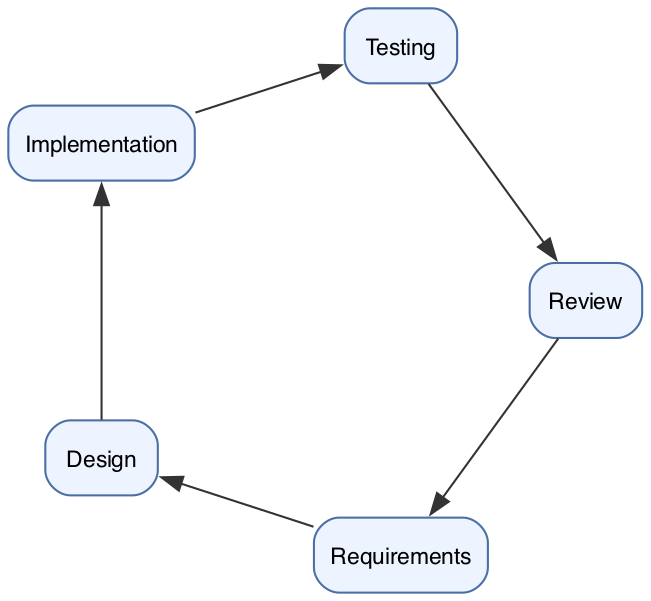
\includegraphics[width=0.55\textwidth]{methodology.png}
  \caption{Agile / iterative development methodology}
  \label{fig:method}
\end{figure}

\section{Report Organization}
This report is organised into several chapters, each describing a specific area of the project:

\textbf{Chapter 1: Introduction} presents an overview of the project, including the problem
statement, objectives, scope, limitations, and methodology.

\textbf{Chapter 2: Background Study and Literature Review} examines the current state of cafe
operations and reviews existing systems and technologies relevant to the project.

\textbf{Chapter 3: System Analysis and Design} describes the requirements, feasibility study,
and the models and diagrams used to design the system.

\textbf{Chapter 4: Implementation and Testing} explains how the design was translated into a
working application and the testing carried out to verify it.

\textbf{Chapter 5: Conclusion and Future Recommendations} summarises the outcomes and proposes
directions for future improvement.

% ======================================================= CHAPTER 2
\chapter{BACKGROUND STUDY AND LITERATURE REVIEW}

\section{Background Study}
Cafes and coffee shops form a large and growing part of the food and beverage industry. Their
operations, however, remain highly manual in many small and medium establishments. Orders are
commonly taken on paper pads, prices are totalled by hand, and stock is checked by physically
inspecting shelves. While these methods are simple, they do not scale well during busy periods
and provide no historical record that can be analysed later.

Digital point-of-sale (POS) and restaurant management solutions exist, but they are frequently
designed for larger restaurants, require dedicated hardware, or come with subscription costs
that are difficult to justify for a small cafe. As a result, many cafe owners continue with
manual processes despite their drawbacks.

This project studies these gaps and proposes a lightweight, browser-based alternative that runs
on existing devices, requires no installation, and focuses on the specific needs of a cafe:
fast ordering, accurate billing, simple inventory control, and clear sales insight.

\section{Literature Review}
This section reviews existing research and systems related to restaurant and cafe automation,
point-of-sale technology, web-based management systems, and usability in small-business
software. The reviewed works establish the gap that CafeFlow addresses and justify the design
decisions taken in this project.

\textbf{1. Point-of-Sale Systems in Food and Beverage.}
Ramos and Castro~\cite{lit_pos} studied point-of-sale (POS) systems in the food and beverage
industry and found that, while such systems deliver clear efficiency gains in order taking and
billing, their real-world benefit depends strongly on user acceptance and ease of use. Their
findings support the central premise of this project, that replacing manual order and billing
workflows with a digital system improves speed and accuracy, while also highlighting that the
interface must be simple enough for staff to adopt. CafeFlow responds to both points by
digitising the order-to-bill workflow behind a clean, role-based interface.

\textbf{2. Web-Based, Layered System Architecture.}
Fielding~\cite{lit_web} formalised the client--server and layered architectural constraints
behind modern web systems, showing that separating user-interface concerns from data-storage
concerns improves portability and scalability and allows components to evolve independently.
CafeFlow adopts exactly this separation: a browser-based React interface communicates over HTTP
with server-side API handlers that sit above a data-access layer, keeping the system
maintainable and accessible from any networked device without local installation.

\textbf{3. Component-Based Front-End Frameworks.}
A comparative study of front-end frameworks~\cite{lit_react} analyses React, Angular, and Vue and
concludes that component-based libraries such as React allow complex, interactive interfaces to
be built efficiently through reusable components and a predictable, state-driven rendering model,
and that framework choice should be a reasoned decision. This is directly relevant to CafeFlow,
whose order-builder, dashboard, and reporting screens are highly interactive and benefit from a
component-based structure with client-side state management.

\textbf{4. Lightweight Embedded Databases.}
Gaffney et al.~\cite{lit_sqlite}, in a study of SQLite, describe it as a serverless,
zero-configuration, fully transactional relational database that is the most widely deployed
database engine in the world and is well suited to embedded and single-application use where the
overhead of a dedicated database server is unjustified. CafeFlow uses SQLite for exactly this
reason: a single cafe outlet needs reliable, ACID-compliant persistence without the cost and
administration of a separate database server.

\textbf{5. Usability and Technology Acceptance.}
Nielsen~\cite{lit_usability} derived a refined set of usability heuristics from a factor analysis
of real usability problems, providing principles such as visibility of system status,
consistency, error prevention, and minimalist design. Complementing this, Davis'
Technology Acceptance Model~\cite{lit_tam} establishes that perceived usefulness and perceived
ease of use are the primary determinants of whether users adopt a system. Together these works
indicate that adoption of small-business software depends heavily on simplicity and clarity;
CafeFlow applies their guidance through a clean, role-based interface, short and consistent
workflows, and accessibility from any browser.

In summary, the reviewed literature consistently shows that digitising cafe operations improves
efficiency but hinges on user acceptance, that layered web architectures improve scalability and
maintainability, that component-based front ends and embedded databases are appropriate
technologies for this class of application, and that usability and perceived usefulness are
decisive for adoption. CafeFlow combines these established findings into a single, focused cafe
management system that is practical for small establishments and addresses the cost and
complexity limitations identified in prior work.

% ======================================================= CHAPTER 3
\chapter{SYSTEM ANALYSIS AND DESIGN}

\section{System Analysis}
System analysis identifies what the system must do and the constraints under which it must
operate. CafeFlow is analysed as a role-based web application with two types of users —
\textbf{Administrator} and \textbf{Staff} — interacting with seven functional modules:
authentication, dashboard, menu, orders, billing, inventory, reporting, and staff management.
The analysis below captures the requirements, feasibility, and models that guided the design.

\section{Requirement Analysis}
\textbf{Functional Requirements:}
\begin{enumerate}
  \item The system shall allow users to log in with an email and password and shall enforce
        role-based access (admin vs.\ staff).
  \item The system shall allow administrators to create, edit, delete, and toggle availability
        of menu items.
  \item The system shall allow staff to build an order from available menu items, set a table
        number and optional customer name, and submit it.
  \item The system shall track each order through pending, preparing, and completed states.
  \item The system shall generate an itemised bill for an order.
  \item The system shall allow administrators to manage inventory items and shall raise
        low-stock alerts.
  \item The system shall allow administrators to add and remove staff members and assign roles.
  \item The system shall compute and display sales analytics (revenue, orders, top items,
        category split) from stored order data.
\end{enumerate}

\textbf{Non-Functional Requirements:}
\begin{enumerate}
  \item \textbf{Security:} Passwords shall be stored as bcrypt hashes and sessions managed with
        secure, HTTP-only cookies.
  \item \textbf{Usability:} The interface shall be clean and responsive, usable on desktop,
        tablet, and mobile.
  \item \textbf{Performance:} Common operations such as loading the menu or submitting an order
        shall complete within a fraction of a second on a local deployment.
  \item \textbf{Reliability:} Data shall be persisted to a SQLite database so that it survives
        restarts.
  \item \textbf{Maintainability:} The code shall be organised into clear layers (UI, API, data
        access) to ease future changes.
\end{enumerate}

\subsection{Feasibility Analysis}
\textbf{Technical Feasibility:} The system is built with well-supported, freely available
technologies (Next.js, React, TypeScript, SQLite), all of which run on standard hardware. The
required skills and tools were available, making the project technically feasible.

\textbf{Operational Feasibility:} The system targets a real, everyday need and offers a simple,
role-based interface that cafe staff can use with minimal training, so it is operationally
feasible.

\textbf{Economic Feasibility:} The project relies entirely on open-source software and runs on
commodity hardware, so development and running costs are minimal, making it economically
feasible.

\textbf{Schedule Feasibility:} The project was divided into small Agile increments with clear
milestones, allowing it to be completed within the available academic timeframe.

\subsection{System Modelling}
The system is modelled using standard UML and process diagrams. The \textbf{use case diagram}
in Figure~\ref{fig:usecase} shows the interactions between the two actors and the system, and
the \textbf{order processing flow} in Figure~\ref{fig:flow} shows the lifecycle of an order
from creation to billing.

\begin{figure}[H]
  \centering
  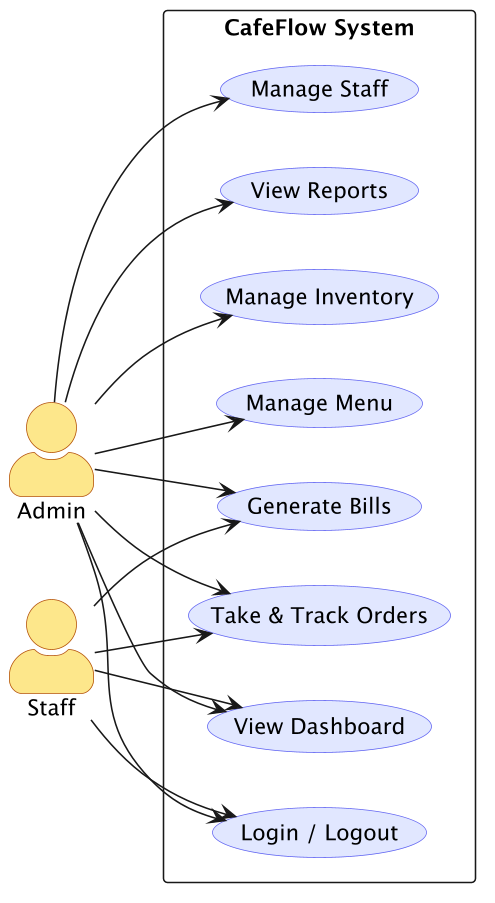
\includegraphics[width=0.62\textwidth]{usecase.png}
  \caption{Use case diagram of CafeFlow}
  \label{fig:usecase}
\end{figure}

\begin{figure}[H]
  \centering
  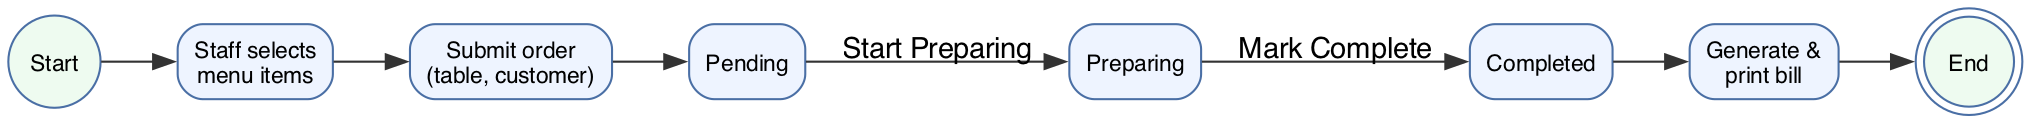
\includegraphics[width=\textwidth]{workflow.png}
  \caption{Order processing flow of CafeFlow}
  \label{fig:flow}
\end{figure}

\section{System Design}
The system design translates the requirements and models into concrete structures: the user
interface, the data model, and the runtime architecture.

\subsection{Interface Design (UI/UX)}
The interface uses a clean, role-based layout with a fixed sidebar for navigation and a content
area for each module. Figure~\ref{fig:login} shows the login screen and Figure~\ref{fig:dash}
shows the administrator dashboard with live statistics and charts.

\begin{figure}[H]
  \centering
  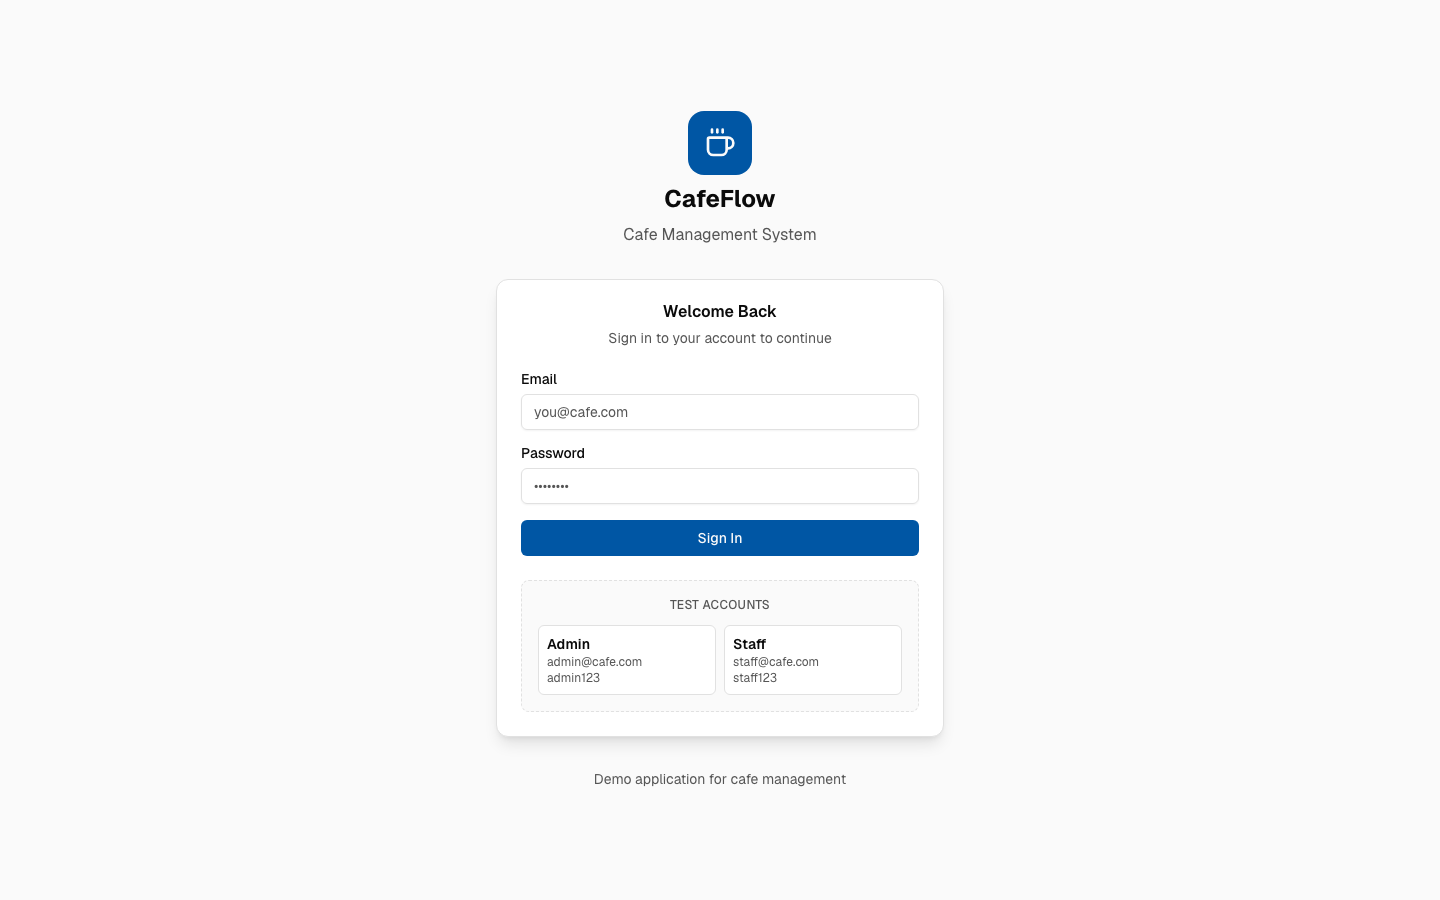
\includegraphics[width=0.6\textwidth]{01-login.png}
  \caption{Login interface of CafeFlow}
  \label{fig:login}
\end{figure}

\begin{figure}[H]
  \centering
  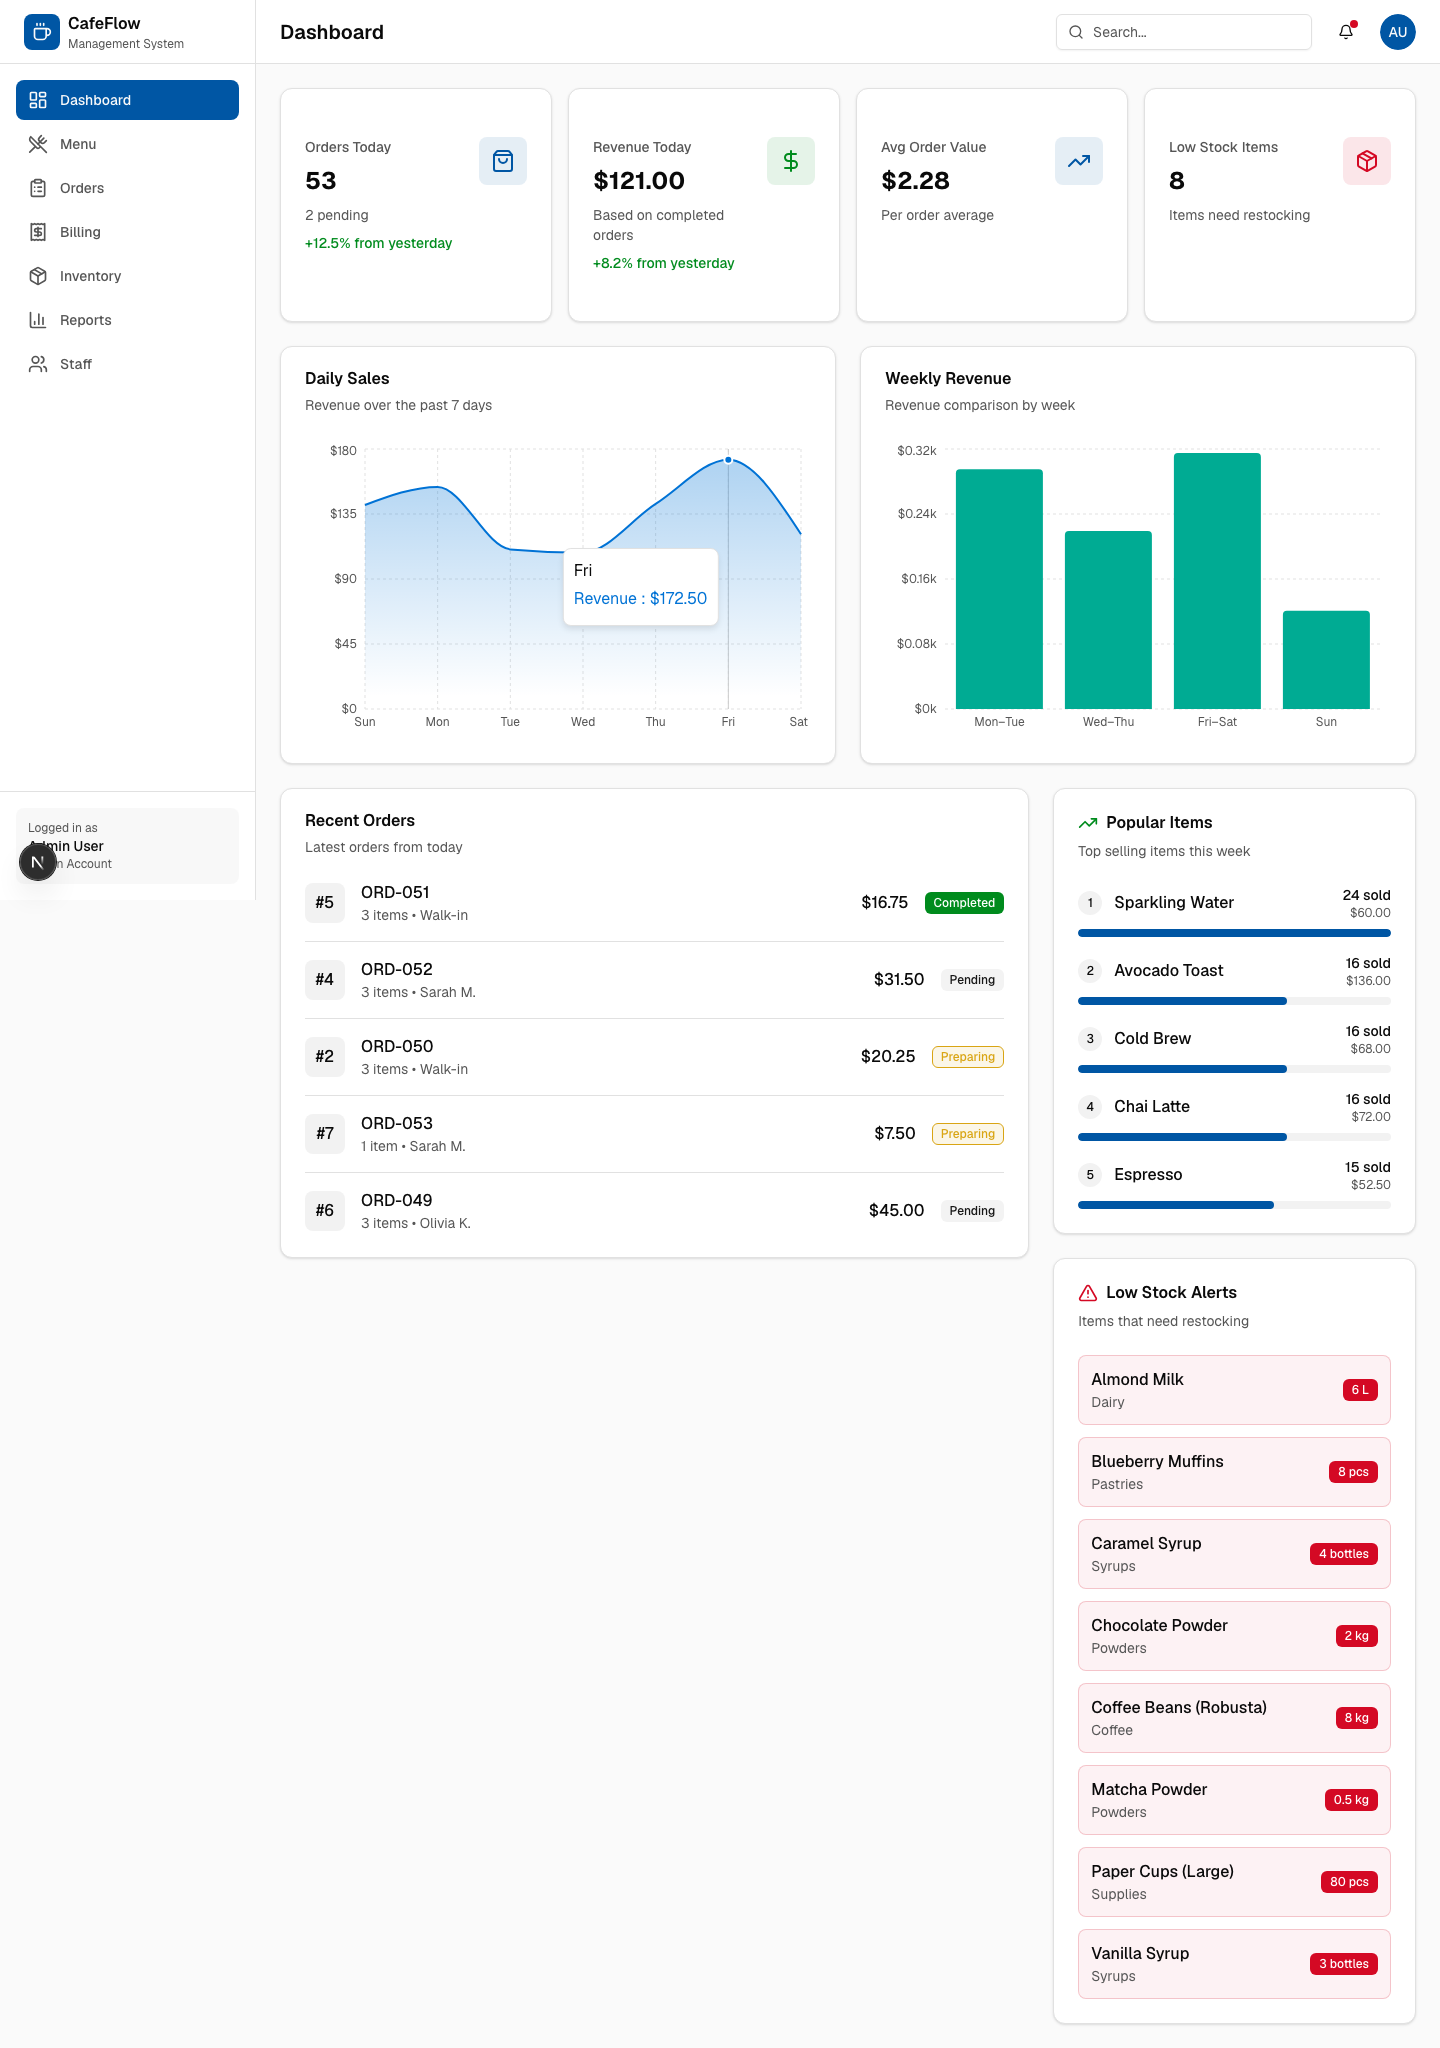
\includegraphics[width=\textwidth]{02-dashboard.png}
  \caption{Administrator dashboard of CafeFlow}
  \label{fig:dash}
\end{figure}

\subsection{Refinement of Classes and Object (Data Model)}
The data is stored in a relational SQLite schema. The \textbf{entity relationship diagram} in
Figure~\ref{fig:er} shows the main tables and their relationships: \texttt{users} and
\texttt{sessions} support authentication; \texttt{menu\_items} and \texttt{inventory\_items}
hold reference data; and \texttt{orders} and \texttt{order\_items} record transactions, with
each order line storing a snapshot of the item name and price so that historical bills remain
correct even if the menu later changes.

\begin{figure}[H]
  \centering
  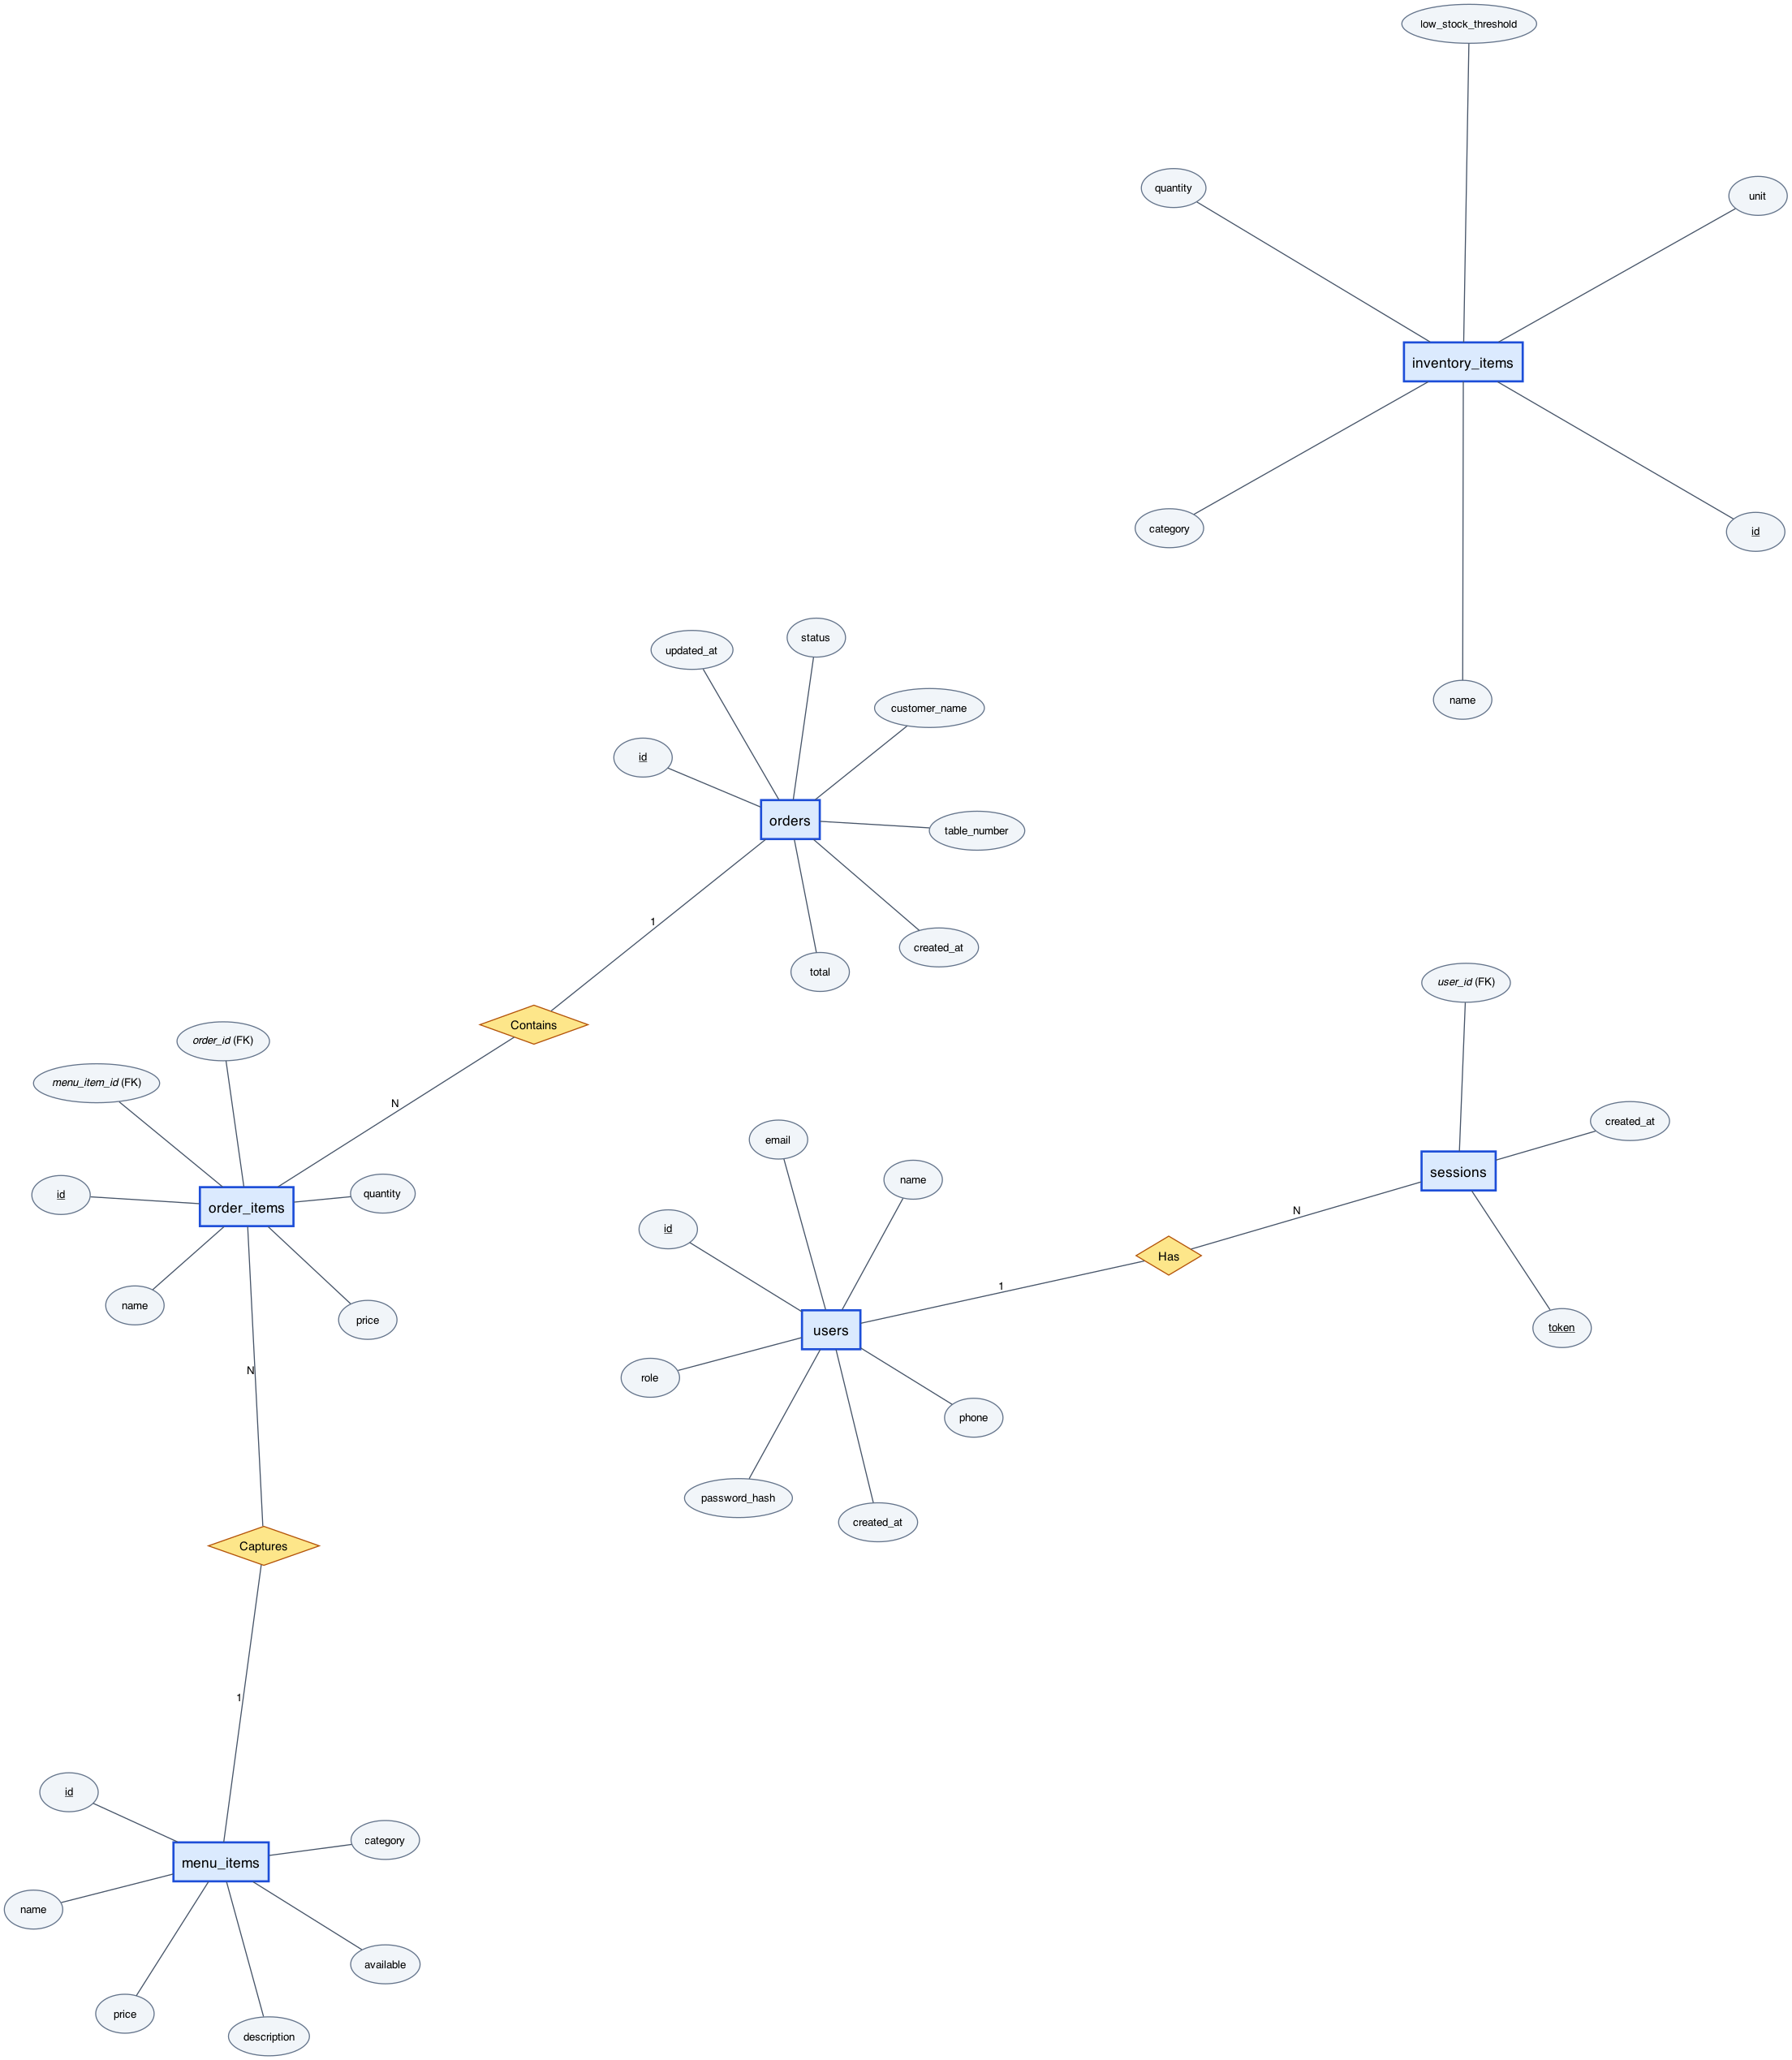
\includegraphics[width=\textwidth]{er.png}
  \caption{Entity relationship diagram of CafeFlow}
  \label{fig:er}
\end{figure}

\subsection{Component Diagram}
The system follows a layered architecture. The browser runs the React user interface and
client-side state stores, which communicate over HTTP with server-side API route handlers.
The handlers apply authentication and authorisation, then use a data-access layer to read and
write the SQLite database. Figure~\ref{fig:arch} shows these components.

\begin{figure}[H]
  \centering
  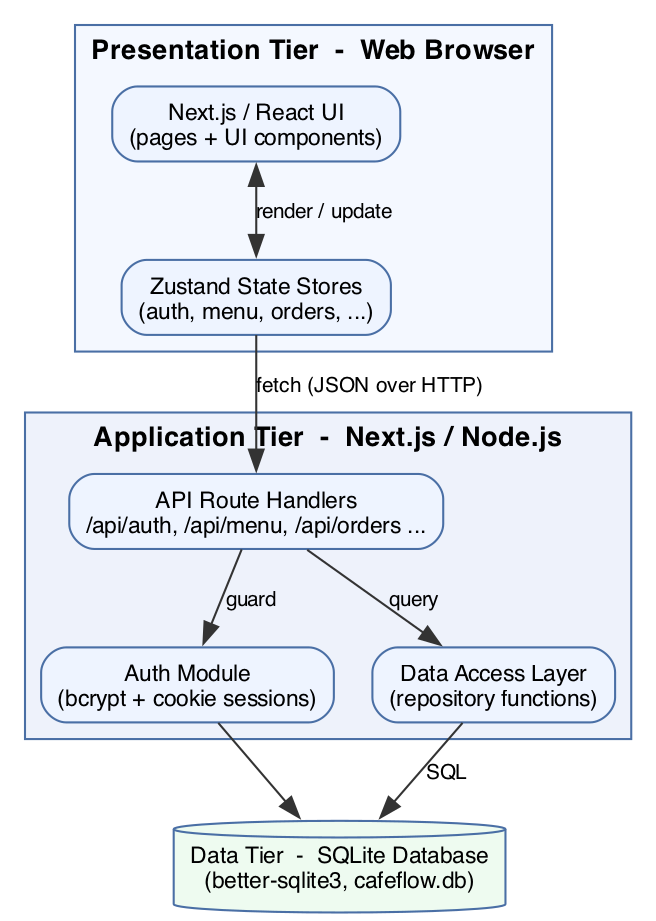
\includegraphics[width=0.85\textwidth]{architecture.png}
  \caption{Component / architecture diagram of CafeFlow}
  \label{fig:arch}
\end{figure}

\subsection{Deployment Diagram}
At runtime the application is deployed as a single Node.js server that serves the Next.js
application and exposes the API, backed by a SQLite database file on the same host. Clients
access the system through a web browser. Figure~\ref{fig:deploy} shows the deployment.

\begin{figure}[H]
  \centering
  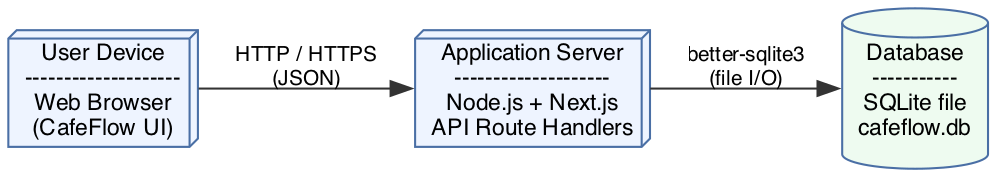
\includegraphics[width=0.9\textwidth]{deployment.png}
  \caption{Deployment diagram of CafeFlow}
  \label{fig:deploy}
\end{figure}

% ======================================================= CHAPTER 4
\chapter{IMPLEMENTATION AND TESTING}

\section{Implementation}
\subsection{Tools Used}
The system was implemented using the following tools and technologies:

\begin{itemize}
  \item \textbf{Next.js \& React:} Full-stack framework and UI library for building the
        application and its API routes.
  \item \textbf{TypeScript:} Typed JavaScript for safer, more maintainable code.
  \item \textbf{Tailwind CSS \& shadcn/ui:} Utility-first styling and accessible UI components.
  \item \textbf{Zustand:} Lightweight client-side state management.
  \item \textbf{SQLite (better-sqlite3):} Embedded relational database for persistence.
  \item \textbf{bcrypt:} Password hashing for secure authentication.
  \item \textbf{Recharts:} Charting library for the dashboard and reports.
  \item \textbf{Playwright:} End-to-end testing framework.
  \item \textbf{Visual Studio Code \& Git/GitHub:} Development environment and version control.
\end{itemize}

\subsection{Implementation Details of Modules}
\textbf{Authentication:} Users sign in with an email and password. Passwords are verified
against bcrypt hashes stored in the \texttt{users} table; on success a session token is stored
in the \texttt{sessions} table and set as a secure HTTP-only cookie. Every protected API
endpoint validates the session, and administrator-only actions additionally check the user's
role.

\textbf{Menu:} Administrators manage menu items through create, edit, delete, and
availability-toggle operations, with search, category filtering, and table/card views.

\textbf{Orders:} Staff build an order by selecting available items, adjusting quantities, and
entering a table number and optional customer name. Submitting an order stores it as
\texttt{pending}; it is then advanced to \texttt{preparing} and \texttt{completed}. Each order
line stores a snapshot of the item name and price.

\textbf{Billing:} Completed and in-progress orders can be selected to produce an itemised bill
showing the cafe header, order details, line items, and total, ready for printing.

\textbf{Inventory:} Stock items are tracked with quantity, unit, category, and a low-stock
threshold. Items at or below their threshold are flagged, and the dashboard shows low-stock
alerts.

\textbf{Staff:} Administrators add and remove team members and assign the admin or staff role.

\textbf{Reports:} Revenue, order counts, average order value, best-selling items, and category
performance are computed from stored order data and presented as summary cards and charts.

\section{Testing}
The system was tested using automated end-to-end tests written with Playwright, which drive a
real browser through the application exactly as a user would. The tests cover every module and
include both unit-level checks of individual functions and system-level checks of complete
workflows. In total, 25 automated tests were executed, all of which passed.

\subsection{Test Cases for Unit Testing}
Table~\ref{tab:unit} lists representative unit test cases that verify individual functions and
behaviours.

\begin{longtable}{|p{1.2cm}|p{4.2cm}|p{4.4cm}|p{2.2cm}|}
\caption{Test Cases for Unit Testing}\label{tab:unit}\\
\hline
\textbf{ID} & \textbf{Test Case} & \textbf{Expected Result} & \textbf{Result} \\ \hline
\endfirsthead
\hline
\textbf{ID} & \textbf{Test Case} & \textbf{Expected Result} & \textbf{Result} \\ \hline
\endhead
\hline
\endfoot
U01 & Login with valid admin credentials & User is authenticated and redirected to dashboard & Pass \\ \hline
U02 & Login with an invalid password & Error message ``Invalid email or password'' is shown & Pass \\ \hline
U03 & Access a protected API without a session & Request is rejected with 401 Unauthorized & Pass \\ \hline
U04 & Add a menu item with valid data & Item is created and appears in the menu list & Pass \\ \hline
U05 & Toggle a menu item's availability & Availability switches and a confirmation is shown & Pass \\ \hline
U06 & Increase an item's quantity in the order cart & Quantity increments and the total updates & Pass \\ \hline
U07 & Add an inventory item & Item is stored and listed in inventory & Pass \\ \hline
U08 & Add a staff member with a duplicate email & Request is rejected with a conflict error & Pass \\ \hline
U09 & Compute order total from line items & Total equals the sum of price $\times$ quantity & Pass \\ \hline
U10 & Reports summary from stored orders & Revenue and order counts are calculated correctly & Pass \\ \hline
\end{longtable}

\subsection{Test Cases for System Testing}
Table~\ref{tab:system} lists system test cases that verify complete, multi-step workflows.

\begin{longtable}{|p{1.2cm}|p{4.2cm}|p{4.4cm}|p{2.2cm}|}
\caption{Test Cases for System Testing}\label{tab:system}\\
\hline
\textbf{ID} & \textbf{Test Case} & \textbf{Expected Result} & \textbf{Result} \\ \hline
\endfirsthead
\hline
\textbf{ID} & \textbf{Test Case} & \textbf{Expected Result} & \textbf{Result} \\ \hline
\endhead
\hline
\endfoot
S01 & Staff signs in and is restricted to permitted sections & Admin-only links (Menu, Reports, Staff) are hidden & Pass \\ \hline
S02 & Staff visits an admin-only route directly & User is redirected back to the dashboard & Pass \\ \hline
S03 & Full menu lifecycle: add, toggle, edit, delete & Each operation succeeds and the list updates & Pass \\ \hline
S04 & Build and submit an order & Order is created and appears under the Pending tab & Pass \\ \hline
S05 & Advance an order pending $\rightarrow$ preparing $\rightarrow$ completed & Status updates at each step with confirmation & Pass \\ \hline
S06 & Generate and print a bill for an order & Itemised bill is shown and print is confirmed & Pass \\ \hline
S07 & Add, edit, and delete an inventory item & Inventory list reflects each change & Pass \\ \hline
S08 & Add a staff member then remove with confirmation & Member is added, then removed after confirming & Pass \\ \hline
S09 & View reports and switch analytics tabs & Summary cards and charts render for each tab & Pass \\ \hline
S10 & Log out & Session ends and the user returns to the login page & Pass \\ \hline
\end{longtable}

\subsection{Result Analysis}
All 25 automated test cases passed, covering authentication and role-based access, menu, order,
billing, inventory, staff, and reporting workflows. The results confirm that the system meets
its functional requirements and behaves correctly across complete user journeys. The automated
suite also serves as a regression guard, allowing future changes to be validated quickly. No
critical defects remained at the end of testing; minor issues found during development (such as
session handling and state updates) were fixed and re-verified.

% ======================================================= CHAPTER 5
\chapter{CONCLUSION AND FUTURE RECOMMENDATIONS}

\section{Conclusion}
CafeFlow successfully delivers a complete, web-based cafe management system that unifies menu
management, order taking, billing, inventory tracking, staff management, and sales reporting in
a single role-based application. By replacing manual, paper-based processes with a fast and
consistent digital workflow, the system reduces service time, improves billing accuracy, and
provides cafe owners with clear, real-time insight into their operations. The project met all
of its stated objectives and was validated by a comprehensive automated test suite.

\section{Lesson Learnt / Outcome}
The project provided valuable experience in designing and building a full-stack web application
end to end. Key lessons included structuring a codebase into clear layers (interface, API, and
data access), securing an application with hashed passwords and session-based authentication,
modelling relational data and preserving historical accuracy through snapshots, and validating
an application thoroughly with automated end-to-end tests. The work also reinforced the value
of an iterative, Agile approach in delivering a working product incrementally.

\section{Future Recommendations}
While CafeFlow meets its current objectives, several enhancements are recommended for the
future:
\begin{enumerate}
  \item \textbf{Online Payments:} Integrate digital wallets and card payment gateways for
        cashless transactions.
  \item \textbf{Multi-Outlet Support:} Extend the system to manage multiple cafe branches from
        a single account.
  \item \textbf{Kitchen Display \& Printing:} Add dedicated kitchen display screens and direct
        thermal-printer support.
  \item \textbf{Customer-Facing Ordering:} Provide QR-code table ordering so customers can place
        orders directly.
  \item \textbf{Advanced Analytics:} Add demand forecasting and automatic stock reorder
        suggestions.
\end{enumerate}

% ======================================================= REFERENCES
\begin{thebibliography}{99}
\addcontentsline{toc}{chapter}{REFERENCES}
\bibitem{lit_pos} Y. Ramos and A. Castro, ``Point-of-sales systems in food and beverage industry: Efficient technology and its user acceptance,'' \textit{Journal of Information Sciences and Computing Technologies}, vol.~6, no.~1, pp.~582--589, 2017.
\bibitem{lit_web} R. T. Fielding, ``Architectural styles and the design of network-based software architectures,'' Ph.D. dissertation, Univ. of California, Irvine, CA, USA, 2000. [Online]. Available: https://roy.gbiv.com/pubs/dissertation/top.htm
\bibitem{lit_react} ``Analysis and comparison of different frontend frameworks,'' in \textit{Applications and Techniques in Information Security (ATIS 2022)}, ser. Communications in Computer and Information Science. Singapore: Springer Nature, 2023, pp.~243--257, doi: 10.1007/978-981-99-2264-2\_19.
\bibitem{lit_sqlite} K. P. Gaffney, M. Prammer, L. Brasfield, D. R. Hipp, D. Kennedy, and J. M. Patel, ``SQLite: Past, present, and future,'' \textit{Proc. VLDB Endowment}, vol.~15, no.~12, pp.~3535--3547, 2022, doi: 10.14778/3554821.3554842.
\bibitem{lit_usability} J. Nielsen, ``Enhancing the explanatory power of usability heuristics,'' in \textit{Proc. SIGCHI Conf. on Human Factors in Computing Systems (CHI '94)}, Boston, MA, USA, 1994, pp.~152--158, doi: 10.1145/191666.191729.
\bibitem{lit_tam} F. D. Davis, ``Perceived usefulness, perceived ease of use, and user acceptance of information technology,'' \textit{MIS Quarterly}, vol.~13, no.~3, pp.~319--340, 1989, doi: 10.2307/249008.
\bibitem{nextjs} Vercel, ``Next.js Documentation,'' [Online]. Available: https://nextjs.org/docs
\bibitem{react} Meta, ``React Documentation,'' [Online]. Available: https://react.dev
\bibitem{ts} Microsoft, ``TypeScript Documentation,'' [Online]. Available: https://www.typescriptlang.org/docs
\bibitem{sqlite} SQLite Consortium, ``SQLite Documentation,'' [Online]. Available: https://www.sqlite.org/docs.html
\bibitem{bsqlite} J. Wiegley, ``better-sqlite3,'' [Online]. Available: https://github.com/WiseLibs/better-sqlite3
\bibitem{tailwind} Tailwind Labs, ``Tailwind CSS Documentation,'' [Online]. Available: https://tailwindcss.com/docs
\bibitem{zustand} pmndrs, ``Zustand,'' [Online]. Available: https://github.com/pmndrs/zustand
\bibitem{playwright} Microsoft, ``Playwright Documentation,'' [Online]. Available: https://playwright.dev
\bibitem{bcrypt} D. Mazi\`eres, ``bcrypt password hashing,'' [Online]. Available: https://en.wikipedia.org/wiki/Bcrypt
\bibitem{recharts} Recharts Group, ``Recharts,'' [Online]. Available: https://recharts.org
\end{thebibliography}

% ======================================================= APPENDICES
\chapter*{APPENDICES}
\addcontentsline{toc}{chapter}{APPENDICES}

The following screenshots show the main modules of the working CafeFlow application.

\begin{figure}[H]
  \centering
  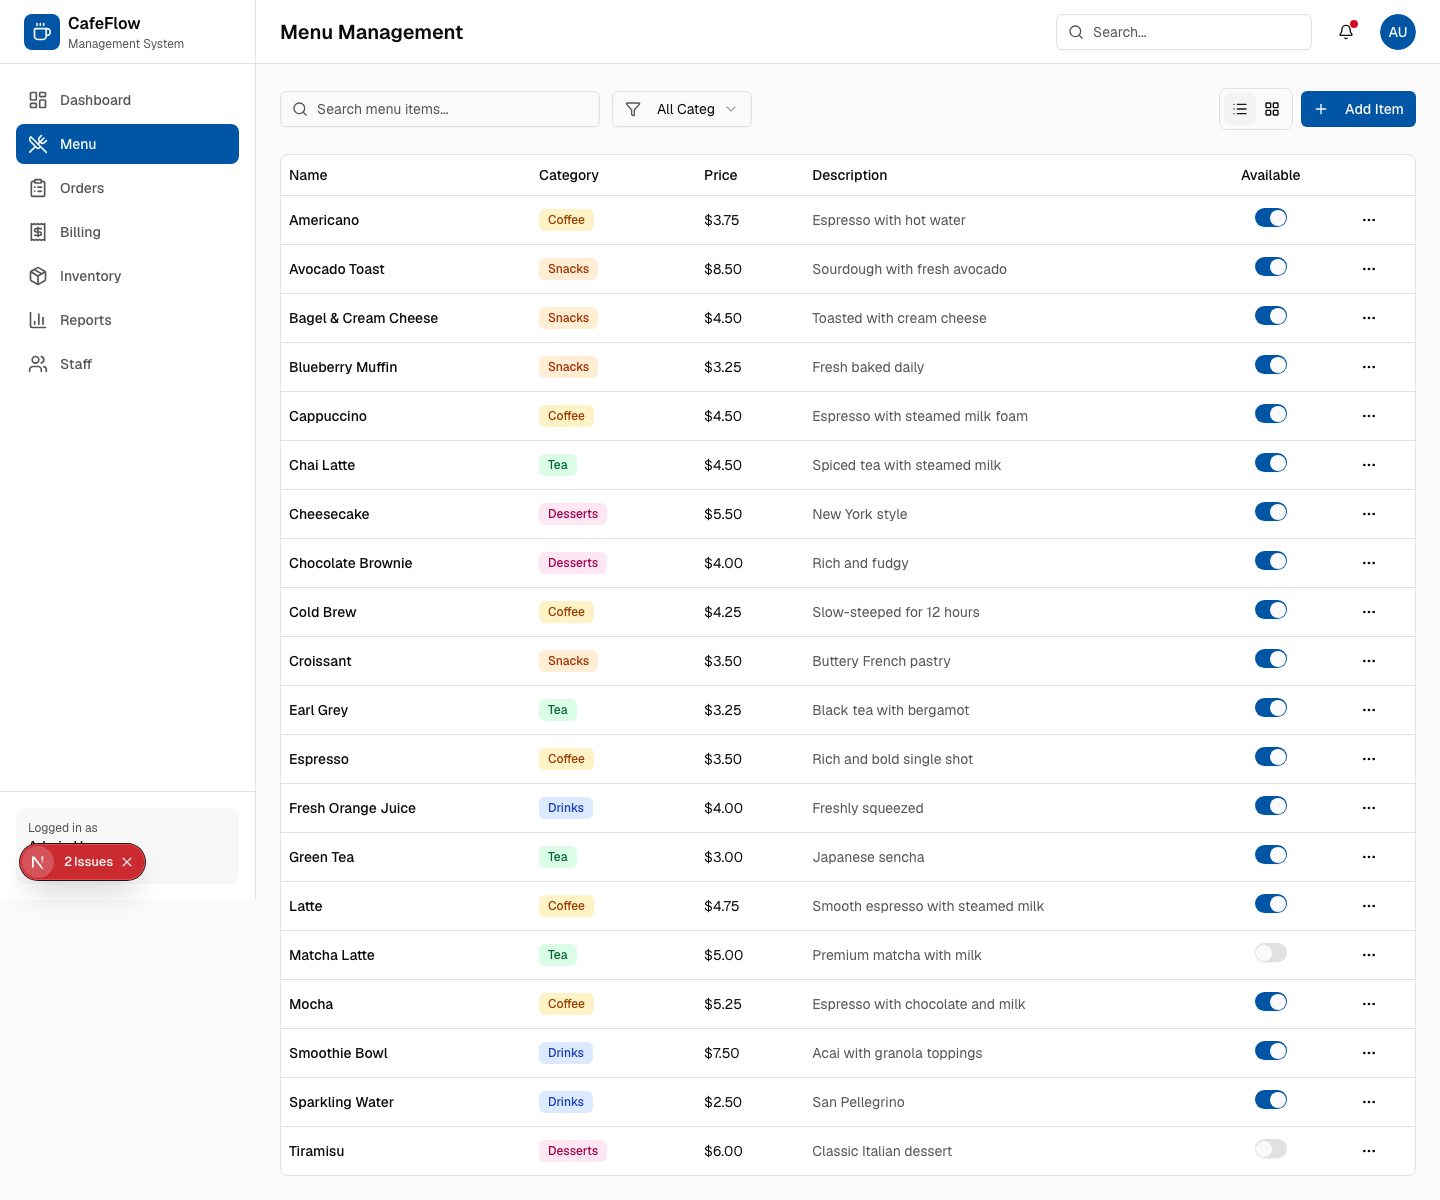
\includegraphics[width=\textwidth]{03-menu.png}
  \caption{Menu management}
\end{figure}

\begin{figure}[H]
  \centering
  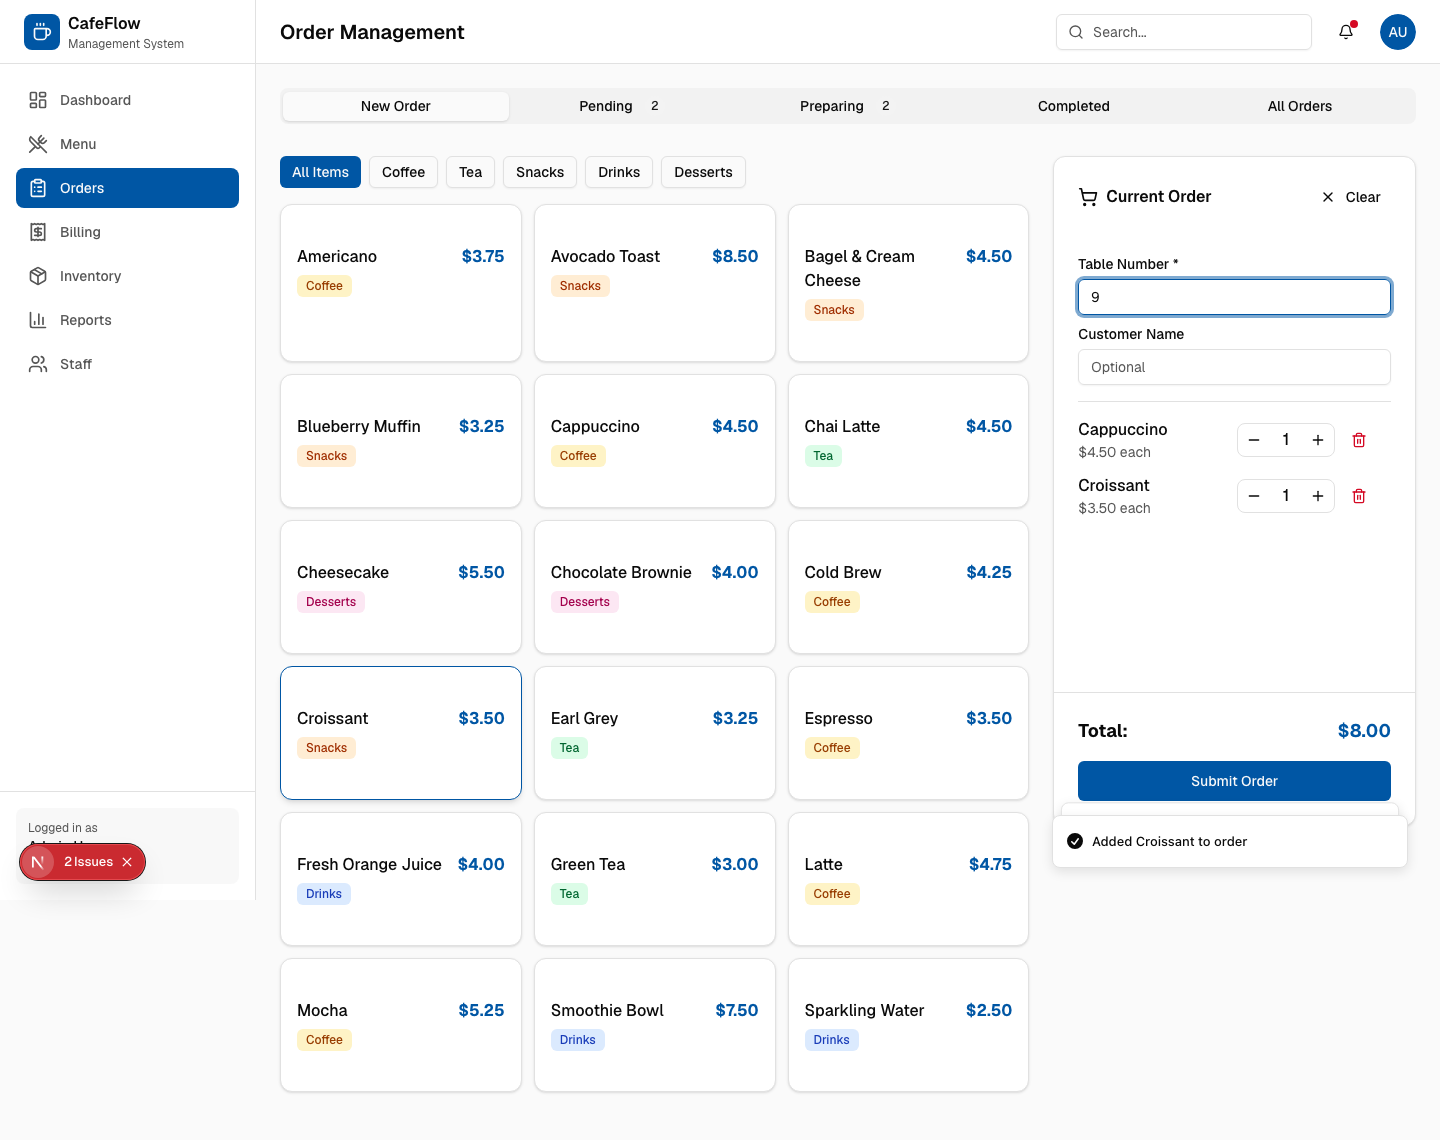
\includegraphics[width=\textwidth]{04-orders-new.png}
  \caption{Order builder (new order)}
\end{figure}

\begin{figure}[H]
  \centering
  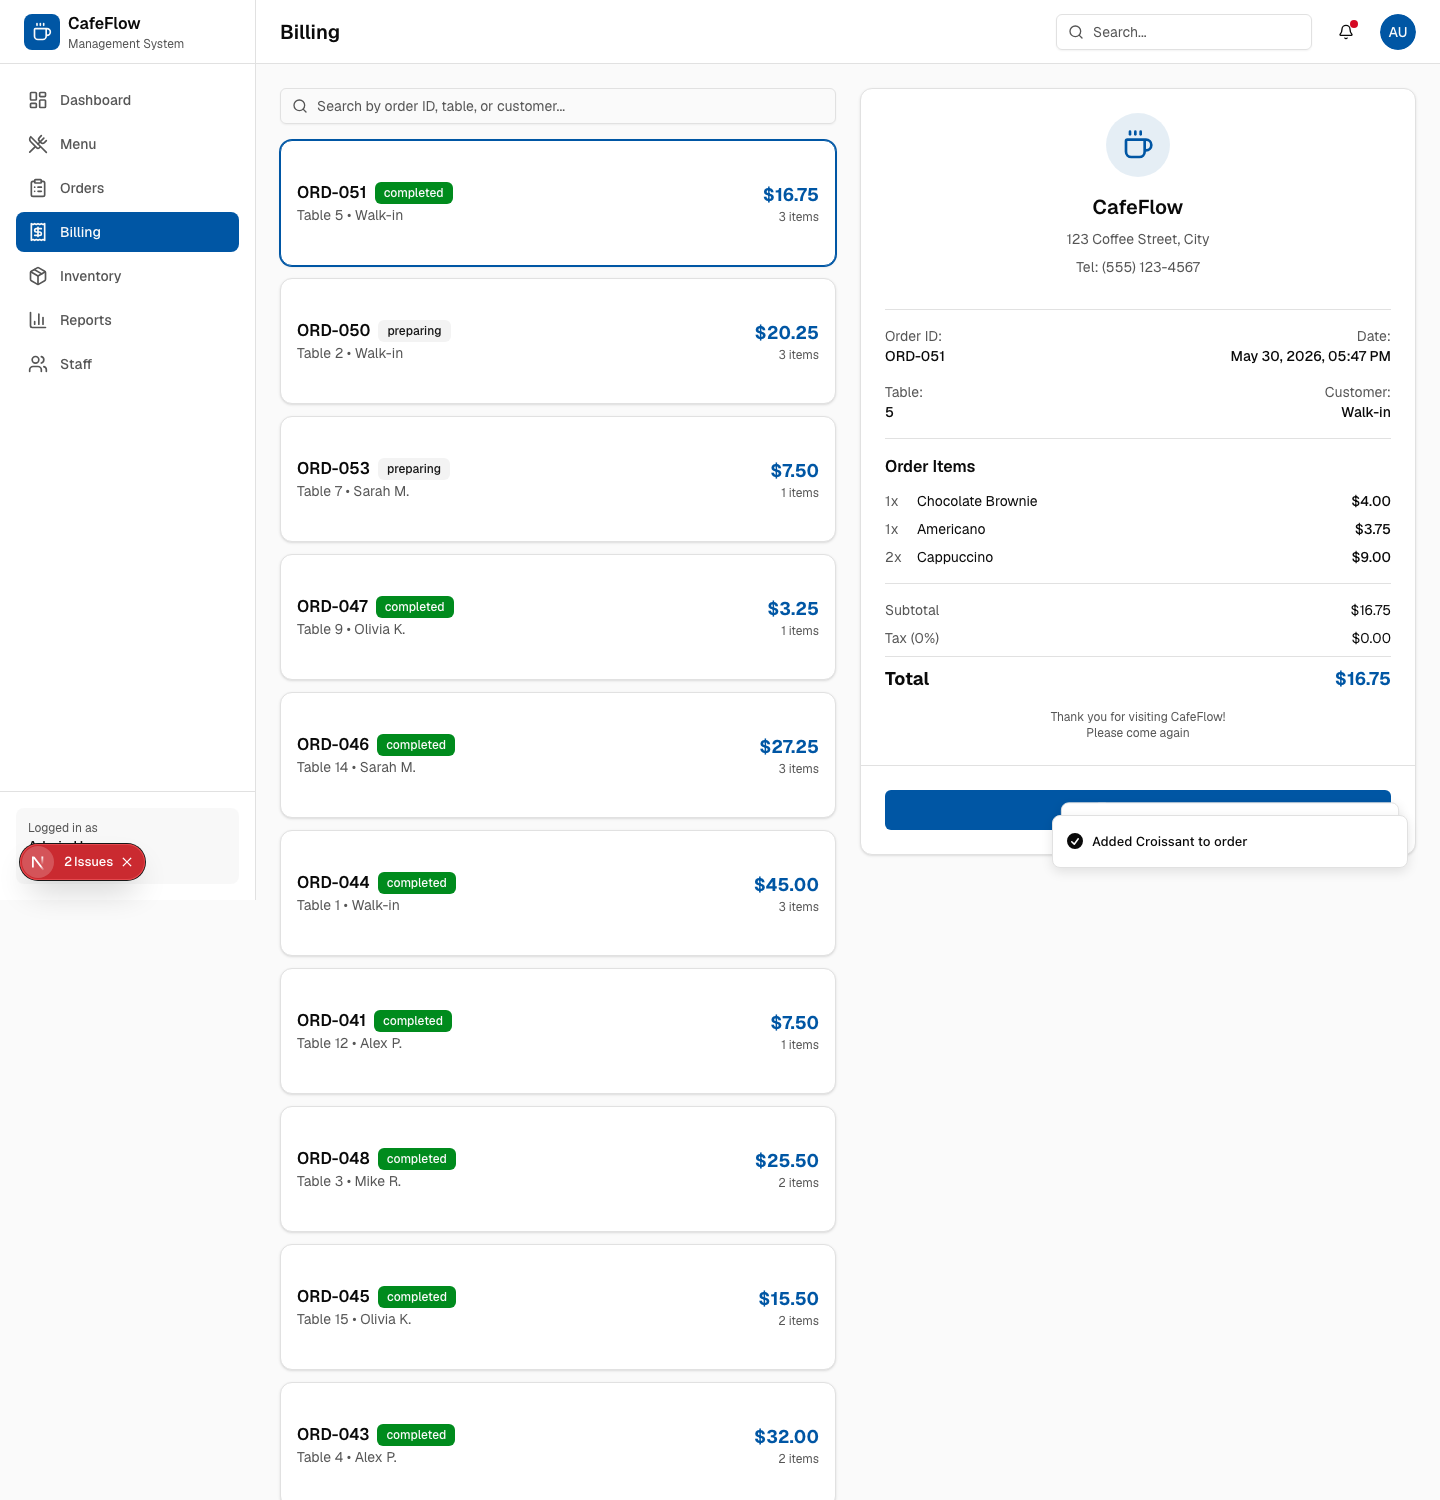
\includegraphics[width=\textwidth]{06-billing.png}
  \caption{Billing and itemised bill preview}
\end{figure}

\begin{figure}[H]
  \centering
  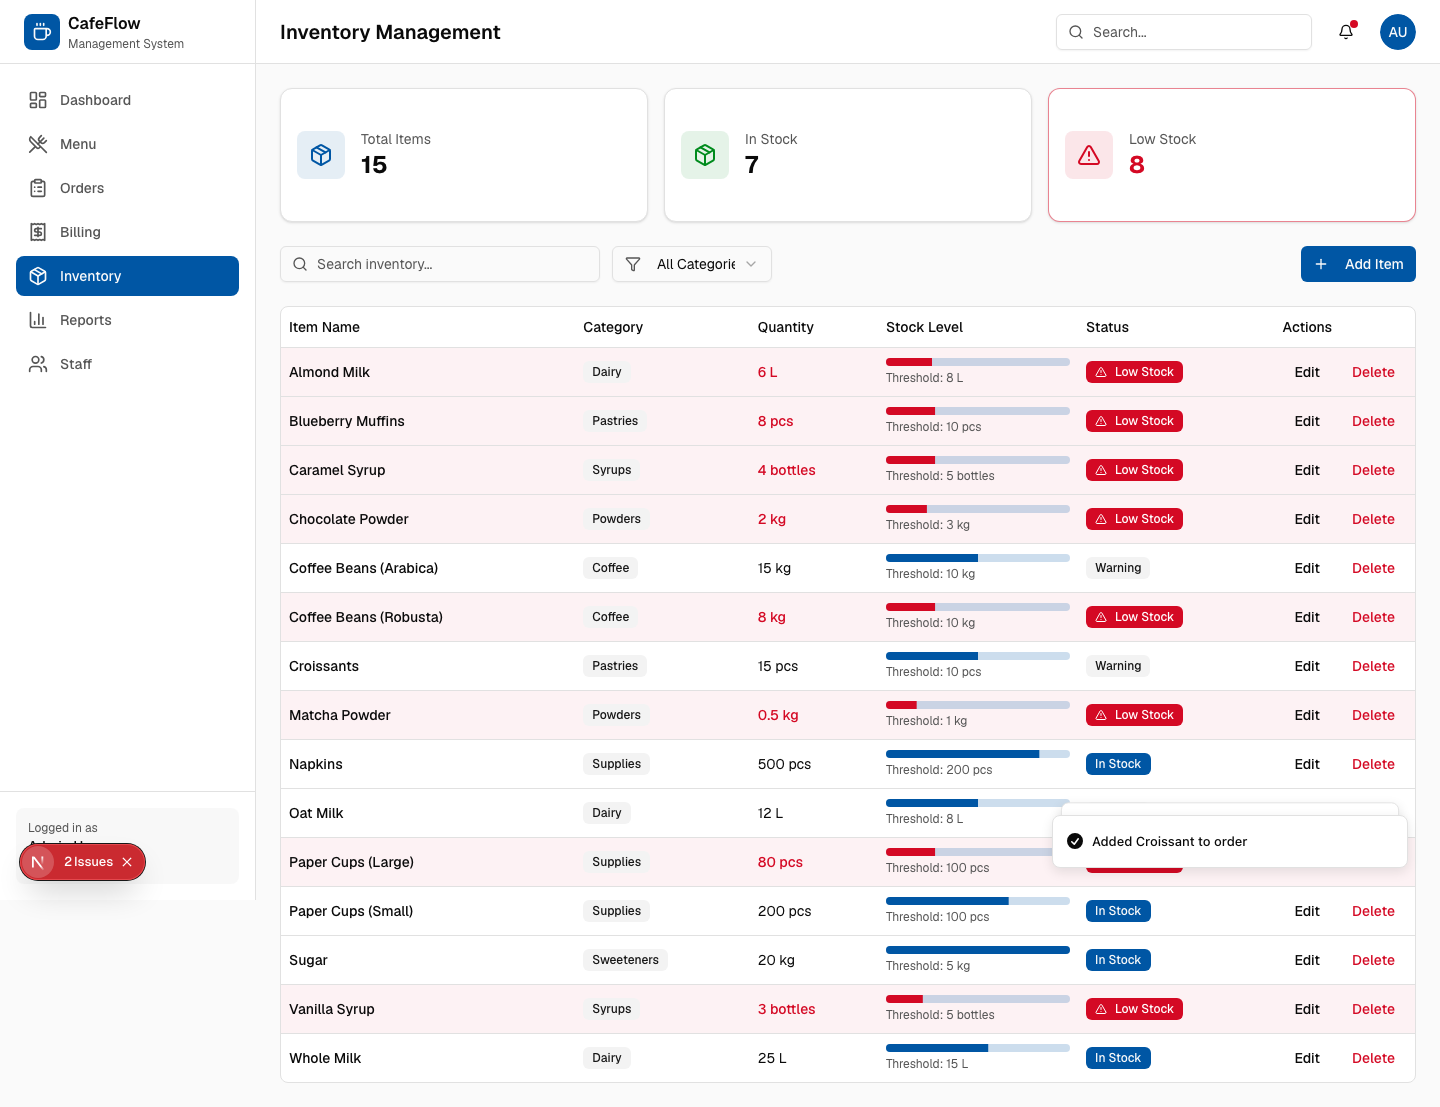
\includegraphics[width=\textwidth]{07-inventory.png}
  \caption{Inventory management}
\end{figure}

\begin{figure}[H]
  \centering
  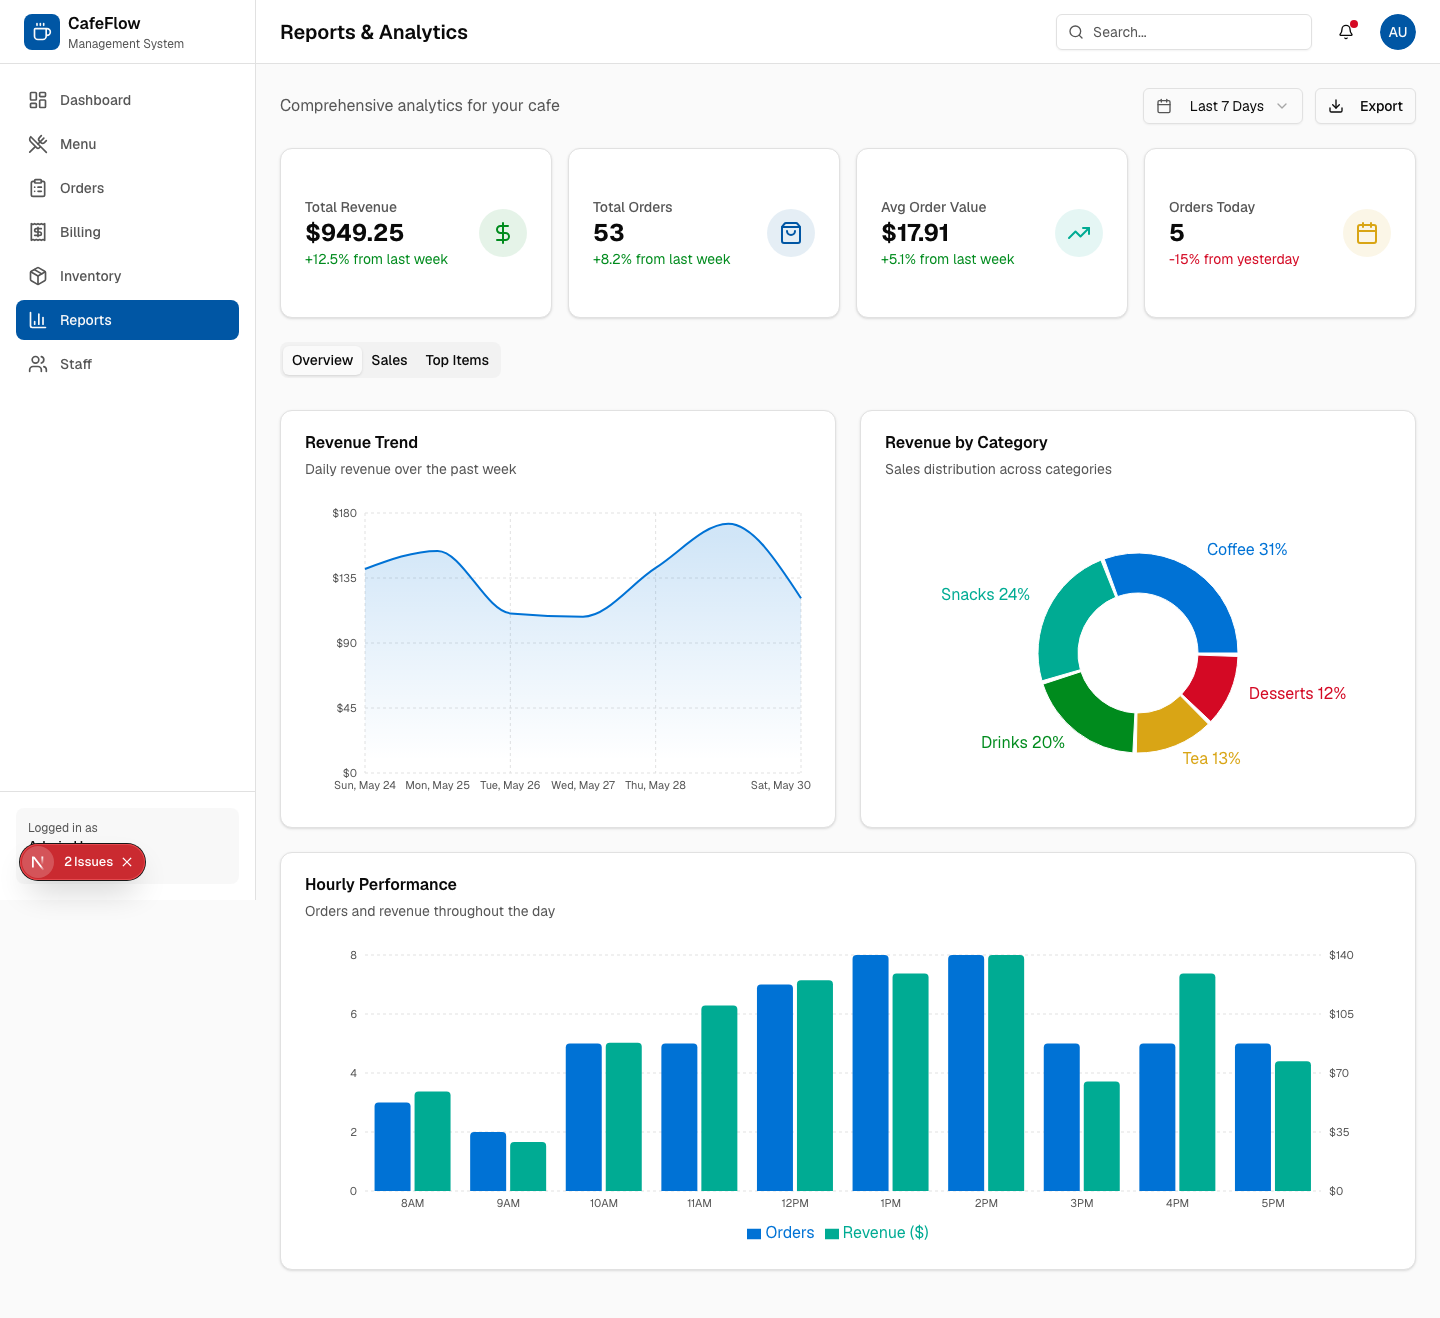
\includegraphics[width=\textwidth]{08-reports.png}
  \caption{Reports and analytics}
\end{figure}

\begin{figure}[H]
  \centering
  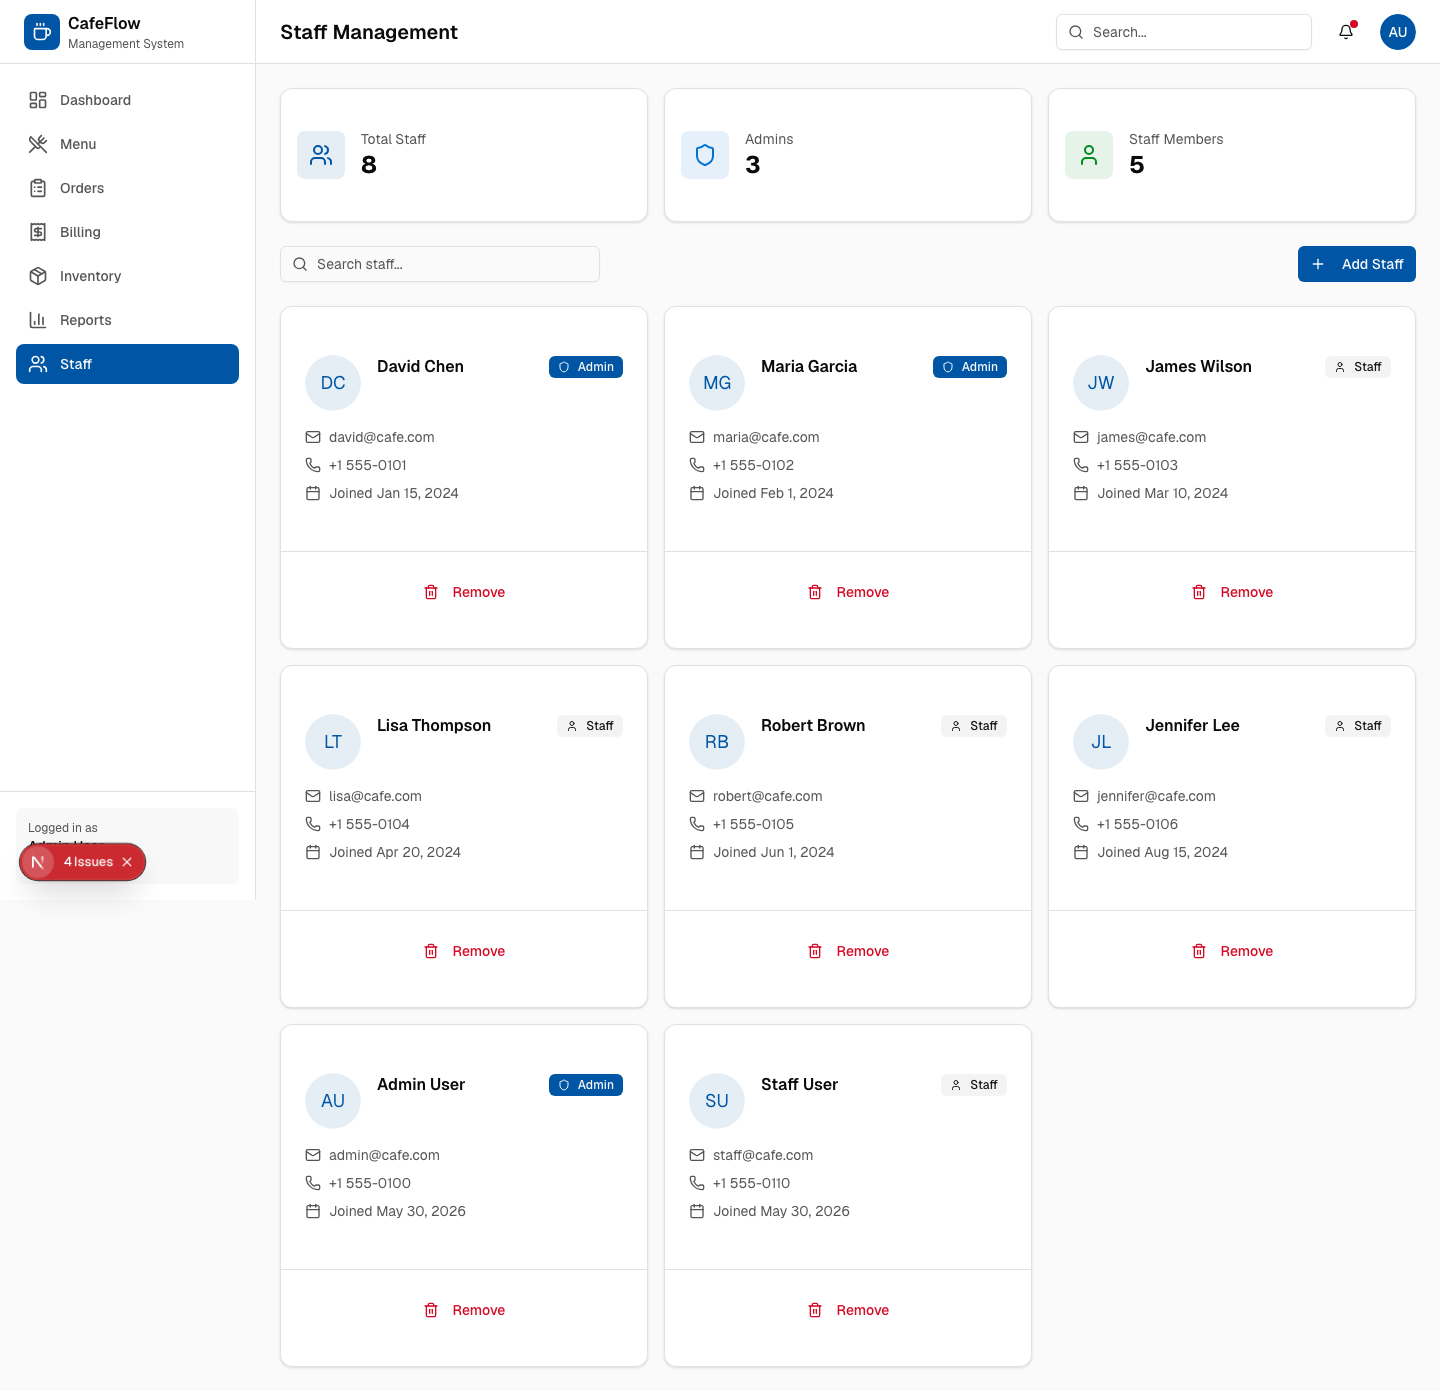
\includegraphics[width=\textwidth]{09-staff.png}
  \caption{Staff management}
\end{figure}

\end{document}
